\documentclass[12pt,a4paper,UTF8]{article}
\usepackage{ctex} % Chinese support
\usepackage{graphicx} % Insert images
\usepackage{subfigure}
\usepackage{float}
\usepackage{listings} % Print source code
\usepackage{color} % Color support
\usepackage{booktabs} % Professional table support
\usepackage{pdflscape} % Landscape pages support in PDF
\usepackage{hyperref} % Hypertext links support for cross-referencing
\usepackage{amsmath,mathtools}
\usepackage{ulem} % strikethrough

% Customize hyperref format (it's set to no special format here)
\hypersetup{hidelinks}

% Declare directories to search for graphics files for graphicx
\graphicspath{{figures/}}

% Define source code style for listings
\lstdefinestyle{verilog-style}{
	language=Verilog,
	basicstyle=\ttfamily\footnotesize,
	keywordstyle=\bfseries\color[rgb]{0, 0, 1},
	identifierstyle=\color[rgb]{0.5, 0.3, 0.1},
	stringstyle=\color[rgb]{0.6, 0.1, 0.1},
	commentstyle=\itshape\color[rgb]{0.05, 0.5, 0.05},
	backgroundcolor=\color[gray]{0.95},
	numbers=left,
	numbersep=5pt,
	numberstyle=\color[gray]{0.6},
	breaklines=true
}

\newcommand{\reporttitle}[2]{
  \LARGE\textsf{#1}\quad\underline{\makebox[12em]{#2}}
}

\newcommand{\reportinfo}[2]{
  \large\makebox[4em]{\textsf{#1}}\quad\underline{\makebox[18em]{#2}}
}

\begin{document}
\begin{titlepage}
  \centering
  \vspace*{\fill}
  {\Huge\textsf{数字电路与数字系统实验}} \\ [100pt]
  \reportinfo{实验名称}{exp10 音频输出实验} \\ [10pt]
  \reportinfo{院系}{计算机科学与技术系} \\ [10pt]
  \reportinfo{学生姓名}{} \\ [10pt]
  \reportinfo{学号}{} \\ [10pt]
  \reportinfo{班级}{数字电路与数字系统实验1班} \\ [10pt]
  \reportinfo{邮箱}{} \\ [10pt]
  \reportinfo{实验时间}{2020 年 11 月 1 日} \\ [10pt]
  \vspace*{\fill}
\end{titlepage}
\tableofcontents
\newpage

\section{实验目的}
\begin{itemize}
  \item 学习如何将数字信号转换为模拟信号
  \item 学习音频信号的输出方式
  \item 复习PS/2键盘控制器的设计方法
  \item \sout{学习乐理知识}
\end{itemize}


\section{实验原理}
本实验的数字音频采用48kHz的采样率,即每间隔1/48000秒
(1/48毫秒的时间产生一个数字输出样本点。对于不同频率
的正弦波信号,其周期对应的样本点数不同。例如对于频率为
960Hz的正弦波,每50个样本点对应它的一个周期。

我们如果要产生不同频率的正弦波,需要先按频率计算出样本点
对应的相位,然后查三角函数表获取对应幅度值的方式。我们存储了
一张1024点的sin函数表。即存储器中以地址k=0$\cdots$1023存储了
1024个三角函数值。我们可以根据频率计算相邻两个样本点所对应的
sin表中的相位之差。然后只需要把这个值传入题目文件提供的模块,
即可生成相应频率的正弦波。


\section{实验环境/器材}
\begin{itemize}
  \item Quartus编辑器和DE10-Standard开发平台
  \item FPGA开发板
  \item 带有PS/2接口的键盘
  \item 带3.5mm接口的耳机
\end{itemize}

\section{程序代码结构}
\begin{figure}[H]
  \centering
  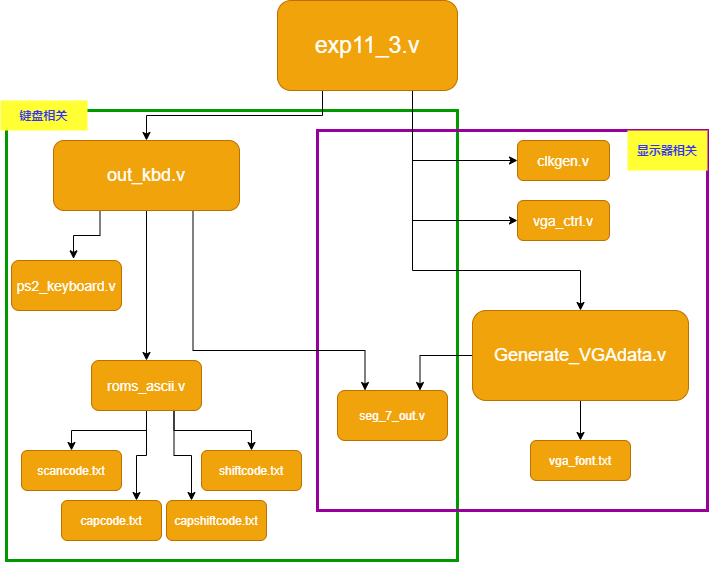
\includegraphics[width=1\textwidth]{code_structure.PNG}
  \caption{模块结构}
  \label{struct}
\end{figure}

\section{实验步骤/过程}
\subsection{键盘控制模块}
编写键盘控制模块的方法和实验8大体相同。通过调用\mbox{ps2\_keyboard}
模块获取扫描码,依次判断当前的按键状态。因为不需要输出键码和ASCII码,
所以我们对实验8的代码进行了一些修改。首先我们要确定应该把什么返回给上层模块。
根据我们要实现的功能,我们发现只需要把当前的按键状态返回即可。所以我们
构建一个八位的变量作为返回值,告诉上层模块哪些琴键处于被按下的状态。

获取按键状态需要对所有通码和断码进行分析。当扫描码读到F0时,说明下一个扫描码
是断码。所以当F0读完时,我们下一个扫描码(即断码)赋给变量\mbox{off\_data},
然后停顿一段时间,直到这个断码读完,再读取下一个通码。通码保存在变量\mbox{eff\_data}
中。
\begin{lstlisting}[style=verilog-style]
always @ (posedge clk) begin
  if (clrn == 0) begin
     nextdata_n <= 1;
     key_off <= 0;
     pressed <= 1;
     eff_data <= 8'b0;
     off_data <= 8'b0;
     cnt_key <= 0;
  end else begin
     if (ready) begin 
        if (data == 8'hF0) begin // don't read F0
           pressed <= 0;
        end else begin
           if (pressed == 0) begin
              pressed <= 1;
              key_off <= 1; // skip break code
              off_data <= data;
              eff_data <= 0;
           end else begin
              if (key_off == 0) eff_data <= data;
           end
        end
        nextdata_n <= 0; 
     end else nextdata_n <= 1;
  
     // delay for next effective code
     if (key_off) begin
        if (cnt_key == 5000000) begin
           cnt_key <= 0;
           key_off <= 0;
        end else begin
           cnt_key <= cnt_key + 1;
           key_off <= 1;
        end
     end 
     
  end
end
\end{lstlisting}

\begin{figure}[H]
  \centering
  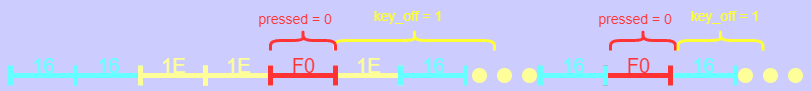
\includegraphics[width=1\textwidth]{scan_code.PNG}
  \caption{控制扫描码}
  \label{scan}
\end{figure}

接着我们就可以根据\mbox{key\_off}信号,再结合通码和断码
来更新按键状态。具体实现在\mbox{kbd\_pressed}模块中,逻辑
很简单,这里就不展示了。

写完键盘控制模块之后不能马上对接音频控制模块,要先测试一下
键盘控制模块运行是否成功。于是我新建一个工程,把按键状态的
八位变量按位赋值给LEDR。操作键盘观察输出得知运行成功。

\begin{figure}[H]
  \centering
  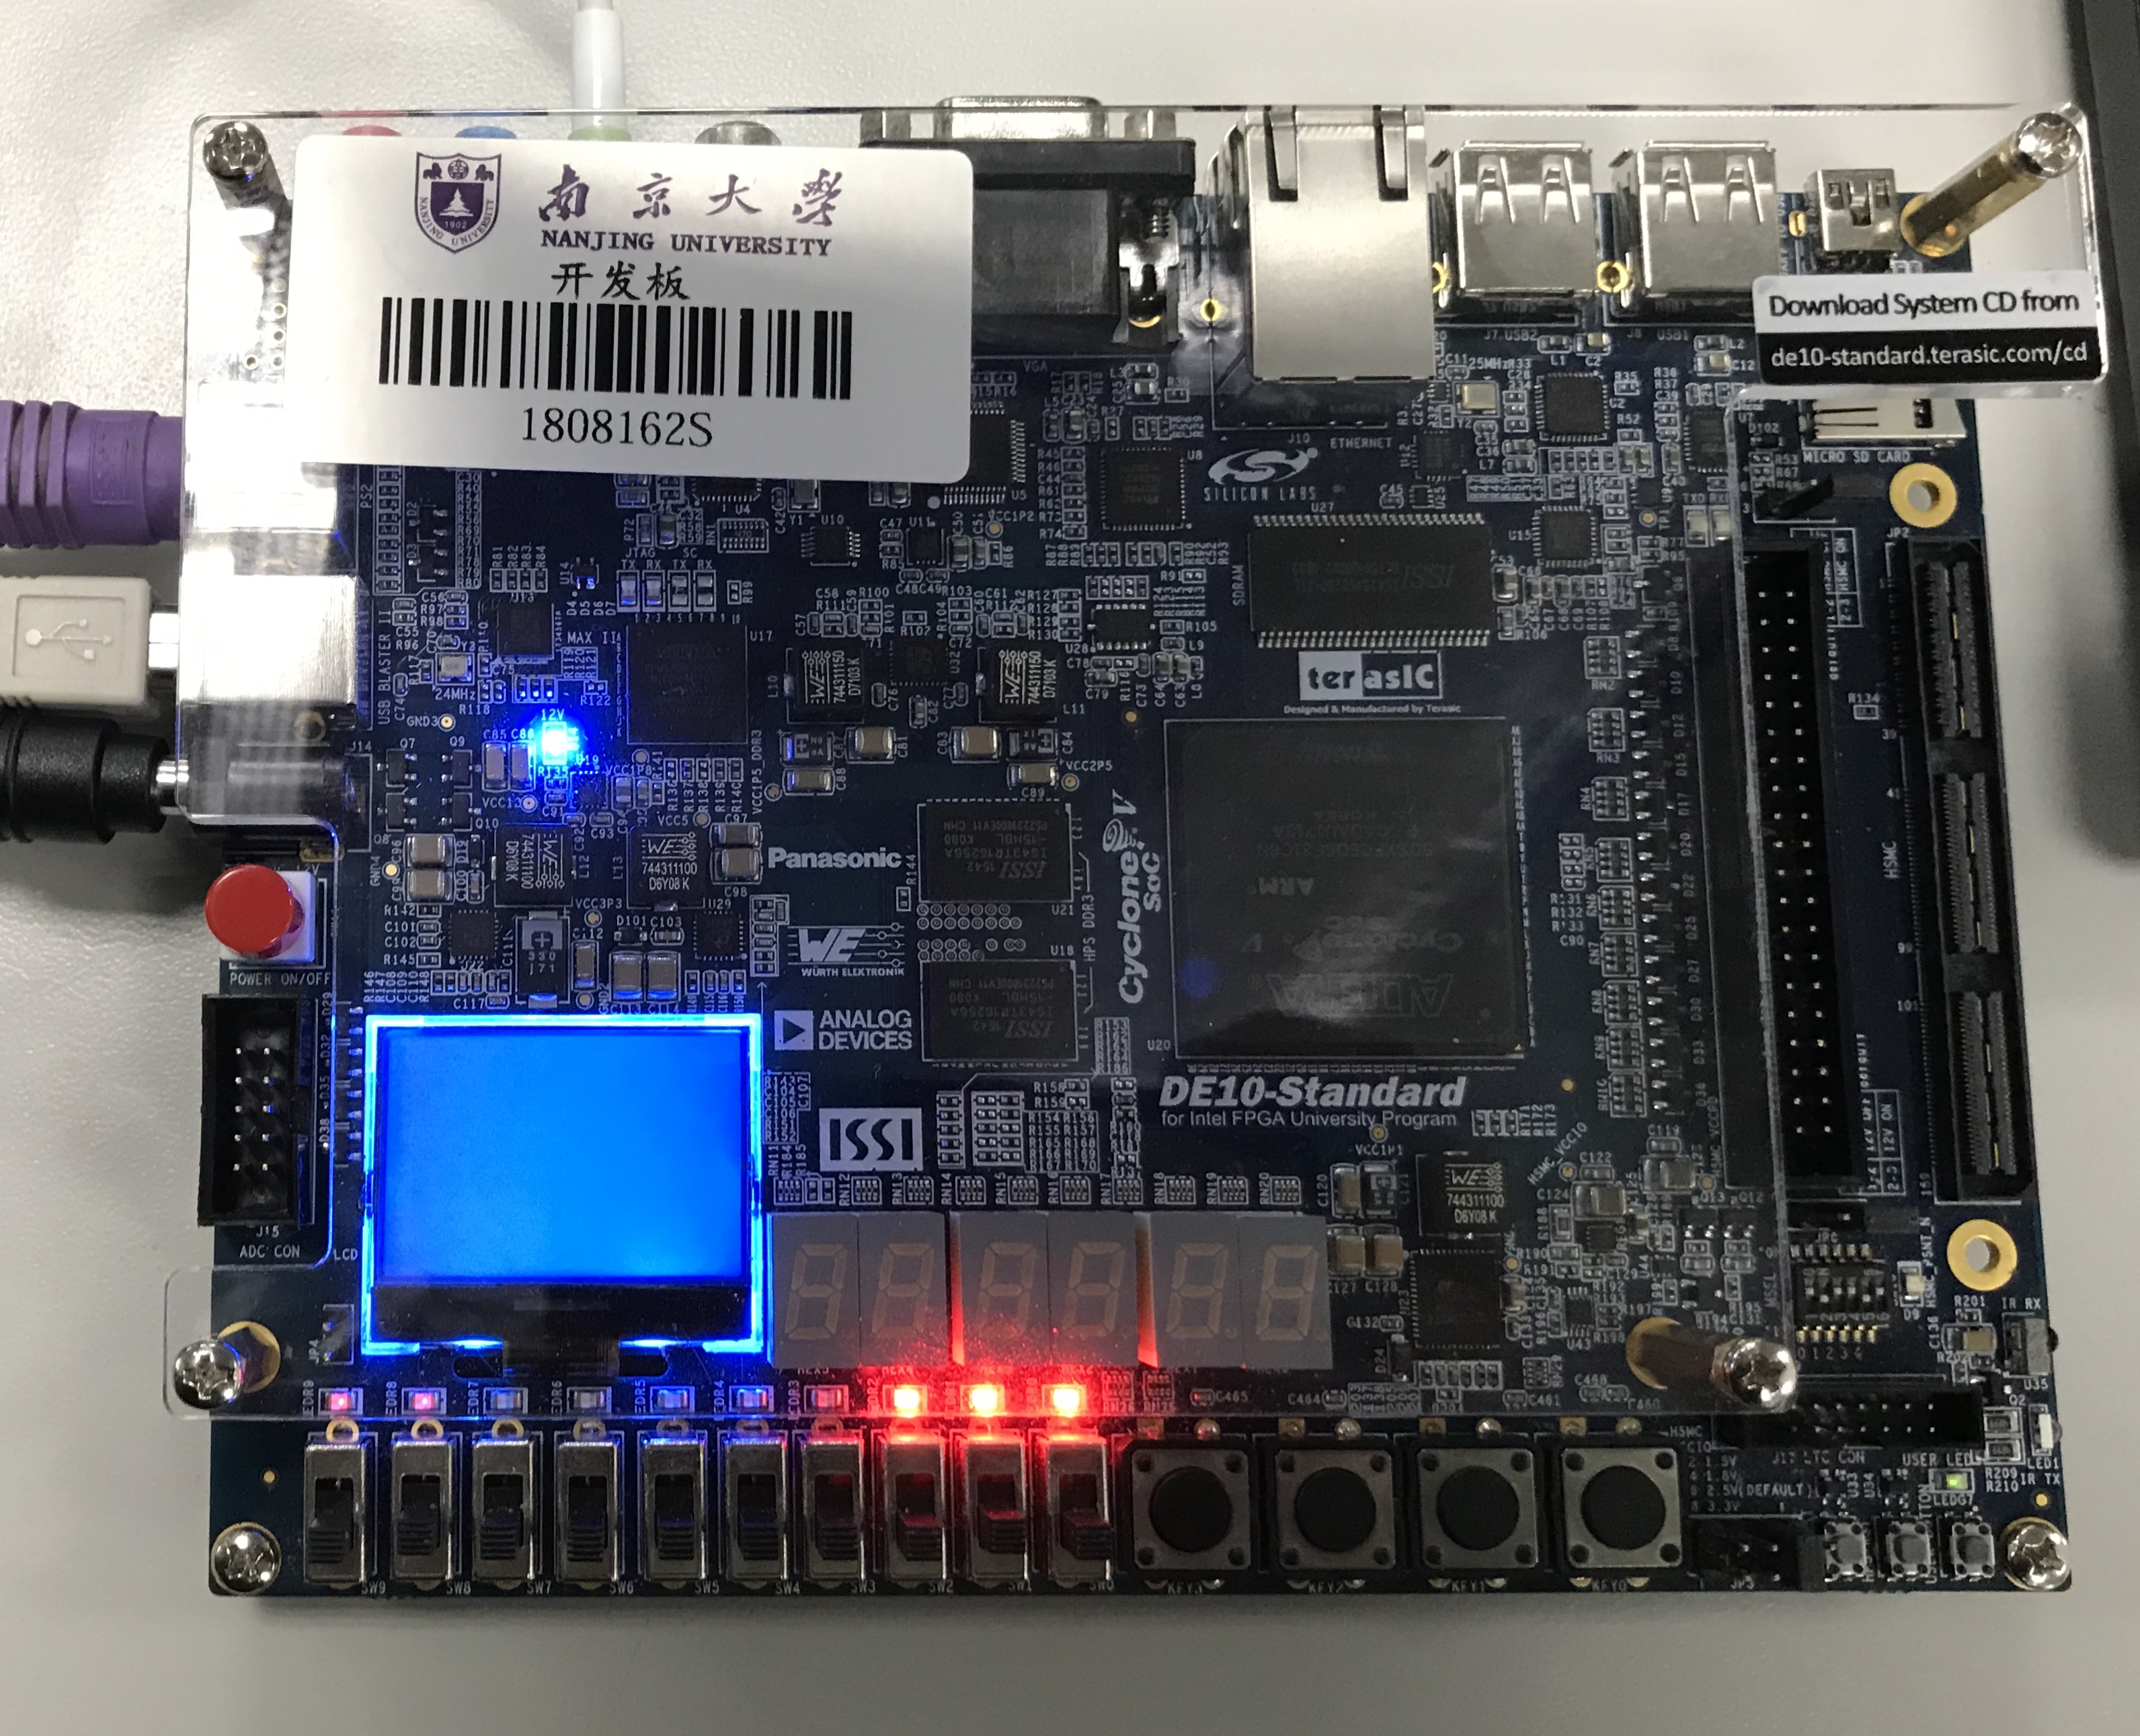
\includegraphics[width=0.8\textwidth]{test_kbd.jpg}
  \caption{同时按do、re、mi}
  \label{kbd}
\end{figure}

\subsection{音符与和声}
在题目提供的工程中,\mbox{Sin\_Generator}模块是在顶层模块中
调用的。在只支持同时按一个键的情况下,我们只需要把该键对应音符的
频率通过简单的计算,传入此模块,即可实现电子琴的单音符输出。于是
我们只需要根据键盘控制模块返回的按键状态,把相应的值传入实现好的
模块,基础功能就实现了。

而和声的实现稍微复杂一些。我们需要把多个键对应的sin值按比例缩小
之后相加,然后把得到的值传给处理sin值的模块。所以我们创建一个名为
\mbox{sin\_processing}的模块,用它调用键盘控制模块和计算sin值的模块,
综合处理按键和对应的sin值,最后返回和声的sin值。

\mbox{Sin\_Generator}的内容不用修改,需要改动的是调用它的上层模块
(从顶层模块改为\mbox{sin\_processing}模块)。我们直接来看
\mbox{sin\_processing}模块:

\begin{lstlisting}[style=verilog-style]
module sin_processing(
    input clk_sys,
    input clk_aud,
    input clrn,
    input ps2_clk,
    input ps2_data, 
    output reg [15:0] final_data
    );
    
    parameter [15:0] freq_do_1 = 16'd714;
    parameter [15:0] freq_re = 16'd802;
    parameter [15:0] freq_mi = 16'd900;
    parameter [15:0] freq_fa = 16'd954;
    parameter [15:0] freq_so = 16'd1070;
    parameter [15:0] freq_la = 16'd1201;
    parameter [15:0] freq_si = 16'd1349;
    parameter [15:0] freq_do_2 = 16'd1429;  
    
    wire [7:0] key_8;
    wire [15:0] freq0, freq1, freq2, freq3, freq4, freq5, freq6, freq7;
    wire [15:0] data0_tmp, data1_tmp, data2_tmp, data3_tmp, data4_tmp, data5_tmp, data6_tmp, data7_tmp;
    wire signed [15:0] data0, data1, data2, data3, data4, data5, data6, data7;
    wire signed [7:0] cnt;
    
    out_kbd kbd1(
       .clk(clk_sys),
       .clrn(clrn),
       .ps2_clk(ps2_clk),
       .ps2_data(ps2_data), 
       .key_8(key_8)
    );
    
    Sin_Generator sin_wave0(.clk(clk_aud), .reset_n(clrn), .freq(freq_do_1), .dataout(data0_tmp));
    Sin_Generator sin_wave1(.clk(clk_aud), .reset_n(clrn), .freq(freq_re), .dataout(data1_tmp));
    Sin_Generator sin_wave2(.clk(clk_aud), .reset_n(clrn), .freq(freq_mi), .dataout(data2_tmp));
    Sin_Generator sin_wave3(.clk(clk_aud), .reset_n(clrn), .freq(freq_fa), .dataout(data3_tmp));
    Sin_Generator sin_wave4(.clk(clk_aud), .reset_n(clrn), .freq(freq_so), .dataout(data4_tmp));
    Sin_Generator sin_wave5(.clk(clk_aud), .reset_n(clrn), .freq(freq_la), .dataout(data5_tmp));
    Sin_Generator sin_wave6(.clk(clk_aud), .reset_n(clrn), .freq(freq_si), .dataout(data6_tmp));
    Sin_Generator sin_wave7(.clk(clk_aud), .reset_n(clrn), .freq(freq_do_2), .dataout(data7_tmp));
 
    assign data0 = key_8[0] ? data0_tmp : 16'd0;
    assign data1 = key_8[1] ? data1_tmp : 16'd0;
    assign data2 = key_8[2] ? data2_tmp : 16'd0;
    assign data3 = key_8[3] ? data3_tmp : 16'd0;
    assign data4 = key_8[4] ? data4_tmp : 16'd0;
    assign data5 = key_8[5] ? data5_tmp : 16'd0;
    assign data6 = key_8[6] ? data6_tmp : 16'd0;
    assign data7 = key_8[7] ? data7_tmp : 16'd0;
    assign cnt = key_8[0]+key_8[1]+key_8[2]+key_8[3]+key_8[4]+key_8[5]+key_8[6]+key_8[7];
    
    initial begin
       final_data = 16'd0;
    end
    
    always @ (posedge clk_aud) begin
       if (clrn == 0 || cnt == 0) begin
          final_data <= 16'd0;
       end else begin
          final_data <= data0/cnt+data1/cnt+data2/cnt
                      +data3/cnt+data4/cnt+data5/cnt
                      +data6/cnt+data7/cnt;
       end
    end
       
 endmodule 
\end{lstlisting}

对于某个音符,它的频率对应的相位递增值(这里直接记为
\mbox{freq\_音符名})是固定的。所以我们可以直接调用
8次\mbox{Sin\_Generator}模块,计算出所有8个音符的
sin值,再根据需要来使用它们。sin值是根据同时按键的键数
按比例缩小的。同时按cnt个键,相应键的sin值就缩小cnt倍,
这样之后再相加就不会溢出了。

\subsection{调节音量}
调节音量是在\mbox{I2C\_Audio\_Config}模块中设置的,
我们需要修改这个模块的内容。修改之前,我们先来研究一下
这个模块是如何工作的(模块内容见题目pdf或题目提供的文件):

此模块的功能是初始化音频设置。它按照一定的时序,依次进行
相关设置(包括音量),所有设置只进行一遍,完成之后不再重新
设置。经过我们的仔细观察,发现音量大小是由存储器的这个单元
进行控制的:

\begin{lstlisting}[style=verilog-style]
audio_reg[3]= 7'h02; audio_cmd[3]=9'h79; //Left Volume
audio_reg[4]= 7'h03; audio_cmd[4]=9'h79; //Right Volume
\end{lstlisting}

于是我们进行相应的修改,使得我们可以用FPGA开发板上的按钮
来设置音量加和音量减。需要注意的是读取完一个音量加减信号后,
需要经过一段时间,再读取下一个音量加减信号。否则会出现按一下
音量加(减)就调到最大(小)音量的情况。整个模块代码如下:

\begin{lstlisting}[style=verilog-style]
module I2C_Audio_Config(clk_i2c,
                        reset_n,
                        I2C_SCLK,
                        I2C_SDAT,
                        testbit,
                        vol_up,
                        vol_down,
                        l_vol,
                        r_vol);
   parameter total_cmd = 9;
   parameter [8:0] init_vol = 9'h48;

   input clk_i2c;  //10k I2C clock
   input reset_n;
   input vol_up, vol_down;

   output I2C_SCLK;
   output [3:0] testbit;
   output [8:0] l_vol, r_vol;
   inout  I2C_SDAT;

   reg [23:0] mi2c_data;
   reg  mi2c_go;
   wire mi2c_end;
   reg  [1:0] mi2c_state;
   //state 0: stop, state 1: sendnext;
   //state 2: wait for finish, state 3:move index
   
   wire [2:0] mi2c_ack;
   wire [7:0] audio_addr;

   reg [3:0] cmd_count;
   reg [6:0] audio_reg [15:0]; //register to write
   reg [8:0] audio_cmd [15:0]; //register content
   
   reg [8:0] curr_vol;
   reg [31:0] vol_cmd_off_cnt;
   reg vol_cmd_off;

initial begin
   audio_reg[0]= 7'h0f; audio_cmd[0]=9'h0; //reset
   audio_reg[1]= 7'h06; audio_cmd[1]=9'h0; //Disable Power Down
   audio_reg[2]= 7'h08; audio_cmd[2]=9'h2; //Sampling Control
   audio_reg[3]= 7'h02; audio_cmd[3]=init_vol; //Left Volume
   audio_reg[4]= 7'h03; audio_cmd[4]=init_vol; //Right Volume
   audio_reg[5]= 7'h07; audio_cmd[5]=9'h1;  //I2S format
   audio_reg[6]= 7'h09; audio_cmd[6]=9'h1;  //Active
   audio_reg[7]= 7'h04; audio_cmd[7]=9'h16; //Analog path
   audio_reg[8]= 7'h05; audio_cmd[8]=9'h06; //Digital path
   curr_vol = init_vol;
   vol_cmd_off     = 0;
   vol_cmd_off_cnt = 32'b0;
end

assign audio_addr={7'b0011010,1'b0}; 
//WM8731 addr, always write
assign testbit = cmd_count[3:0];

assign l_vol = audio_cmd[3];
assign r_vol = audio_cmd[4];

I2C_Controller u0(.CLOCK(clk_i2c), //	Controller Work Clock
                  .I2C_SCLK(I2C_SCLK),  // I2C CLOCK
                  .I2C_SDAT(I2C_SDAT),  // I2C DATA
                  .I2C_DATA(mi2c_data), // DATA:[SLAVE_ADDR,SUB_ADDR,DATA]
                  .GO(mi2c_go),   // GO transfor
                  .END(mi2c_end),	// END transfor 
                  .ACK(mi2c_ack),	// ACK
                  .RESET_N(reset_n)	);	
						
always @ (posedge clk_i2c or negedge reset_n) begin
   if(!reset_n) begin
      audio_reg[0]<= 7'h0f; audio_cmd[0]<=9'h0;
      audio_reg[1]<= 7'h06; audio_cmd[1]<=9'h0;
      audio_reg[2]<= 7'h08; audio_cmd[2]<=9'h2;
      audio_reg[3]<= 7'h02; audio_cmd[3]<=init_vol;
      audio_reg[4]<= 7'h03; audio_cmd[4]<=init_vol;
      audio_reg[5]<= 7'h07; audio_cmd[5]<=9'h1;
      audio_reg[6]<= 7'h09; audio_cmd[6]<=9'h1;
      audio_reg[7]<= 7'h04; audio_cmd[7]<=9'h16;
      audio_reg[8]<= 7'h05; audio_cmd[8]<=9'h06;
      curr_vol        <= init_vol;
      vol_cmd_off     <= 0;
      vol_cmd_off_cnt <= 32'b0;
      cmd_count       <= 4'b0;
      mi2c_state      <= 2'b0;
      mi2c_go         <= 1'b0;
   end else begin
      if (vol_cmd_off) begin
         if (vol_cmd_off_cnt == 32'd1000) begin
            vol_cmd_off <= 0;
            vol_cmd_off_cnt <= 32'b0;
         end else begin
            vol_cmd_off_cnt <= vol_cmd_off_cnt + 1;
         end
      end
  
      if ((vol_up || vol_down)
         && vol_cmd_off == 0
         && curr_vol + vol_up - vol_down >= 9'h0
         && curr_vol + vol_up - vol_down <= 9'h7f) 
      begin
         audio_reg[0]<= 7'h0f; audio_cmd[0]<=9'h0;
         audio_reg[1]<= 7'h06; audio_cmd[1]<=9'h0;
         audio_reg[2]<= 7'h08; audio_cmd[2]<=9'h2;
         audio_reg[3]<= 7'h02; audio_cmd[3]<=curr_vol + vol_up - vol_down;
         audio_reg[4]<= 7'h03; audio_cmd[4]<=curr_vol + vol_up - vol_down;
         audio_reg[5]<= 7'h07; audio_cmd[5]<=9'h1;
         audio_reg[6]<= 7'h09; audio_cmd[6]<=9'h1;
         audio_reg[7]<= 7'h04; audio_cmd[7]<=9'h16;
         audio_reg[8]<= 7'h05; audio_cmd[8]<=9'h06;
         curr_vol        <= curr_vol + vol_up - vol_down;
         vol_cmd_off     <= 1;
         vol_cmd_off_cnt <= 32'b0;
         cmd_count       <= 4'b0;
         mi2c_state      <= 2'd0;
      end
        
      case(mi2c_state)
      2'd0: begin  //stop
         if(cmd_count ==4'b0)
            mi2c_state <= 2'd1;
      end
      2'd1: begin
         mi2c_data <= {audio_addr, audio_reg[cmd_count], audio_cmd[cmd_count]};
         mi2c_go   <= 1'b1;
         mi2c_state<= 2'd2;
      end
      2'd2: begin
         if(mi2c_end) begin
            mi2c_state <= 2'd3;
            mi2c_go    <= 1'b0;
         end
      end
      2'd3: begin
         cmd_count <= cmd_count + 4'd1;
         if(cmd_count + 4'd1 < total_cmd)
            mi2c_state <= 2'd1;  //start next
         else
            mi2c_state <= 2'd0;  //last cmd
      end
      endcase
   end  
end
endmodule
\end{lstlisting}

每次调整音量时,都需要用initial块中的初始化语句
重新初始化存储器的原因,详见条目``遇到的问题及解决办法''。


\section{测试方法+实验结果}
此实验写不了test bench,只能用人耳判断实验结果了。
但是有些功能比如音量大小是可以输出检验的。
\begin{figure}[H]
  \centering
  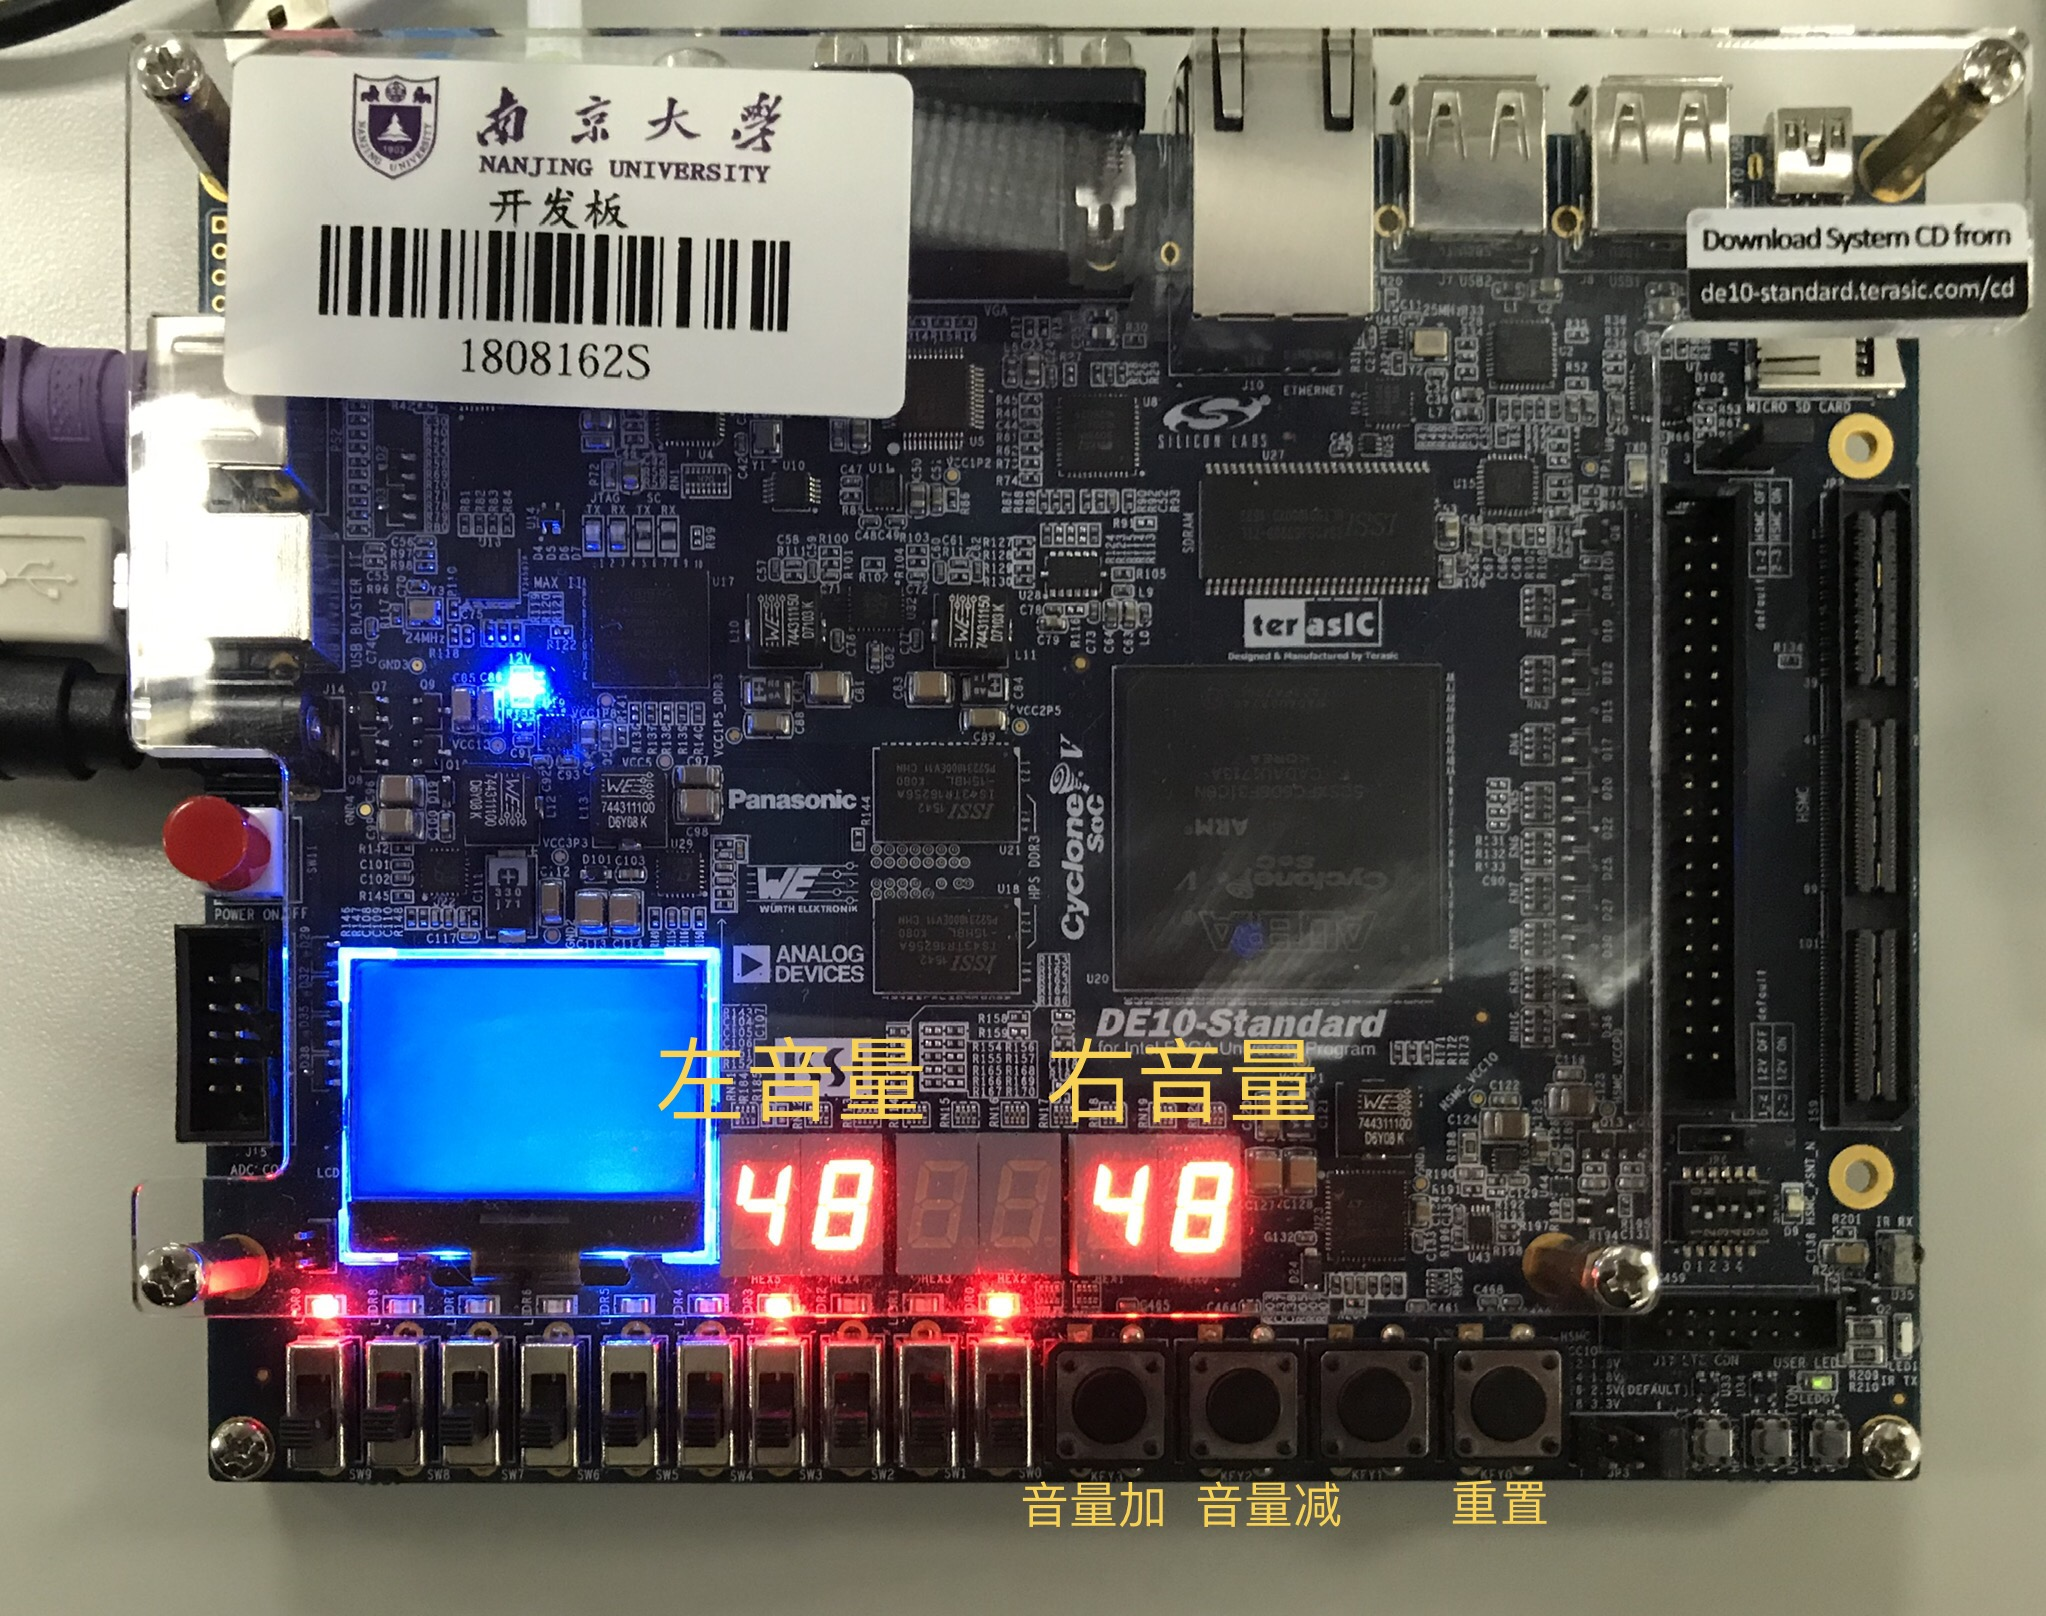
\includegraphics[width=0.8\textwidth]{volume.jpg}
  \caption{FPGA开发板的运行结果}
  \label{fpga}
\end{figure}

测试完毕,实验10完成。

\section{遇到的问题及解决办法}
\begin{itemize}
  \item 在键盘控制模块中,遇到断码时要把\mbox{eff\_data}
        置为0,否则当断码发送完毕后\mbox{eff\_data}仍然是
        该键的键码,该键的按键状态不会改变成未按下的状态。
  \item sin值相加是以有符号数的形式相加,该表达式中的所有
        操作数都必须是有符号数的形式
  \item \fbox{未知原因的bug}在调节音量的模块中,如果用
        题目提供的文件,并把音量对应的存储器单元输出到
        七段数码管上。我们会发现,该单元的值竟然变成了0。
        也就是说,在初始化音频设置完成后,存储器的内容可能
        丢失了。所以在我们自己实现的音量调节代码中,每次
        设置都会重新为存储器赋值,以保证能正常调节音量
\end{itemize}

\section{得到的启示}
\begin{itemize}
  \item 声音也是一种编码。数字不仅可以表示有形的事物,也可以
        表示无形的事物
  \item \sout{在机房一晚上解决不了的bug,躺在床上半小时就能想出原因}
  \item \sout{我宣布我就是心算带师}
\end{itemize}

\section{意见和建议}
\begin{itemize}
  \item 实验提供的代码文件\mbox{I2C\_Audio\_Config.v}中,
        在reset部分给\mbox{mi2c\_state}赋的值应是\mbox{2'b0}
        而不是\mbox{4'b0}
\end{itemize}

\end{document}